\section{Pregunta 2}

En este problema se diseñarán distintos tipos de controladores para una planta no lineal, que obedece a la siguiente dinámica:

\begin{align}
y(k) = \left(0.9 - \frac{0.4}{\sqrt{1 + [y(k - 2)]^2}}\right) y(k - 1) - \left(0.5 + \frac{0.7}{\sqrt{1 + [y(k - 1)]^2}}\right) y(k - 2) \\
+ u(k - 1) - 0.3u(k - 2) + 0.2u(k - 1)u(k - 2) + \epsilon(k)
\end{align}

donde \(\epsilon(k)\) es un ruido blanco gaussiano con media \(0\) y varianza \(\sigma^2 = (0.01)^2\). Además, la planta tiene un tiempo de muestreo de \(T_s = 1 \; [s]\). Se requiere diseñar diferentes tipos de controladores, por lo que:

\begin{enumerate}
    \item \textbf{Diseñe un controlador PI clásico utilizando como referencia la señal \(r(t) = 2\). Los requisitos de diseño del controlador son los siguientes:}
    \begin{itemize}
        \item Sobrespaso menor al 10\%.
        \item Tiempo de estabilización menor a 100 \([s]\).
    \end{itemize}
    
    Para la simulación del sistema se utilizará la herramienta \textit{Simulink}. Primero, es necesario implementar la planta no lineal del sistema mediante el bloque \textit{MATLAB Function}, que se muestra en la Figura \ref{fig:1}.
    
    \begin{figure}
        \centering
        \includegraphics[width=1\textwidth]{img/Figure_1}
        \caption{Implementación de la planta no lineal en \textit{Simulink}, junto con el código implementado para la planta, además de las diferentes entradas y salidas.}
        \label{fig:1}
    \end{figure}
    
    Con base en la función implementada en el bloque \textit{MATLAB Function}, se observa que existen 5 entradas: dos de ellas corresponden al retardo de la señal de control \(u(k-1)\) y \(u(k-2)\); otras dos están asociadas a la señal de salida de la planta \(y(k-1)\) y \(y(k-2)\); y finalmente, la señal de ruido blanco \(\epsilon(k)\), implementada mediante una función de ruido blanco gaussiano con media 0 y varianza \(\sigma^2 = (0.01)^2\).
    
    \begin{figure}
        \centering
        \includegraphics[width=0.3\textwidth]{img/Figure_2}
        \caption{Implementación del ruido blanco gaussiano considerando una media de 0, una varianza de \(\sigma^2 = (0.01)^2\), y un tiempo de muestreo de \(T_s = 1 \; [s]\), usando el bloque \textit{band limited white noise}.}
        \label{fig:2}
    \end{figure}
    
    A continuación, se plantea el siguiente esquema general para la implementación del controlador PI, utilizando el bloque \textit{PID Controller} de \textit{Simulink}. Además, la entrada de referencia corresponde a un escalón \textit{Step} con la forma \(r(t) = 2\), como se muestra en la Figura \ref{fig:3}.
    
    \begin{figure}
        \centering
        \includegraphics[width=0.7\textwidth]{img/Figure_3}
        \caption{Implementación del controlador PI en \textit{Simulink} junto con la señal de referencia \(r(t) = 2\), además de las diferentes entradas y salidas del controlador.}
        \label{fig:3}
    \end{figure}
    
    Con el bloque del controlador PI discreto, se ajustan los parámetros asociados a la ganancia proporcional \(K_p\) y la ganancia integral \(K_i\), obteniéndose los siguientes valores:
    
    \begin{figure}
        \centering
        \includegraphics[width=0.7\textwidth]{img/Figure_5}
        \caption{Implementación del controlador PI en \textit{Simulink} con sus valores de ganancia proporcional \(K_{p} = 0.01\) y ganancia integral \(K_{i} = 0.06\).}
        \label{fig:4}
    \end{figure}
    
    Finalmente, se obtiene la salida de la planta controlada, que se muestra a continuación:
    
    \begin{figure}
        \centering
        \includegraphics[width=0.6\textwidth]{img/Figure_4}
        \caption{Salida de la planta controlada, la cual cumple con el tiempo de establecimiento menor a 100 \([s]\) además de no superar el límite del 10\% de sobrepaso.}
        \label{fig:5}
    \end{figure}
    
    En conclusión, el controlador PI diseñado cumple con los requisitos especificados en cuanto al tiempo de estabilización y el límite de sobrepaso, y su implementación es simple y eficiente.
    \newpage
    \item \textbf{Diseñe un controlador PI difuso considerando 3 conjuntos difusos para cada premisa y para cada consecuencia en la construcción de las reglas.}
    
    Se busca realizar un controlador PI difuso, para lo cual se considerará la misma estructura de la planta mostrada anteriormente en la Figura \ref{fig:1}. Para la implementación del controlador difuso se utilizará el bloque \textit{Fuzzy Logic} de \textit{Simulink}. A continuación, se muestra la implementación del controlador difuso en \textit{Simulink} junto con la señal de referencia \(r(t) = 2\), además de las diferentes entradas y salidas del controlador.
    
    \begin{figure}
        \centering
        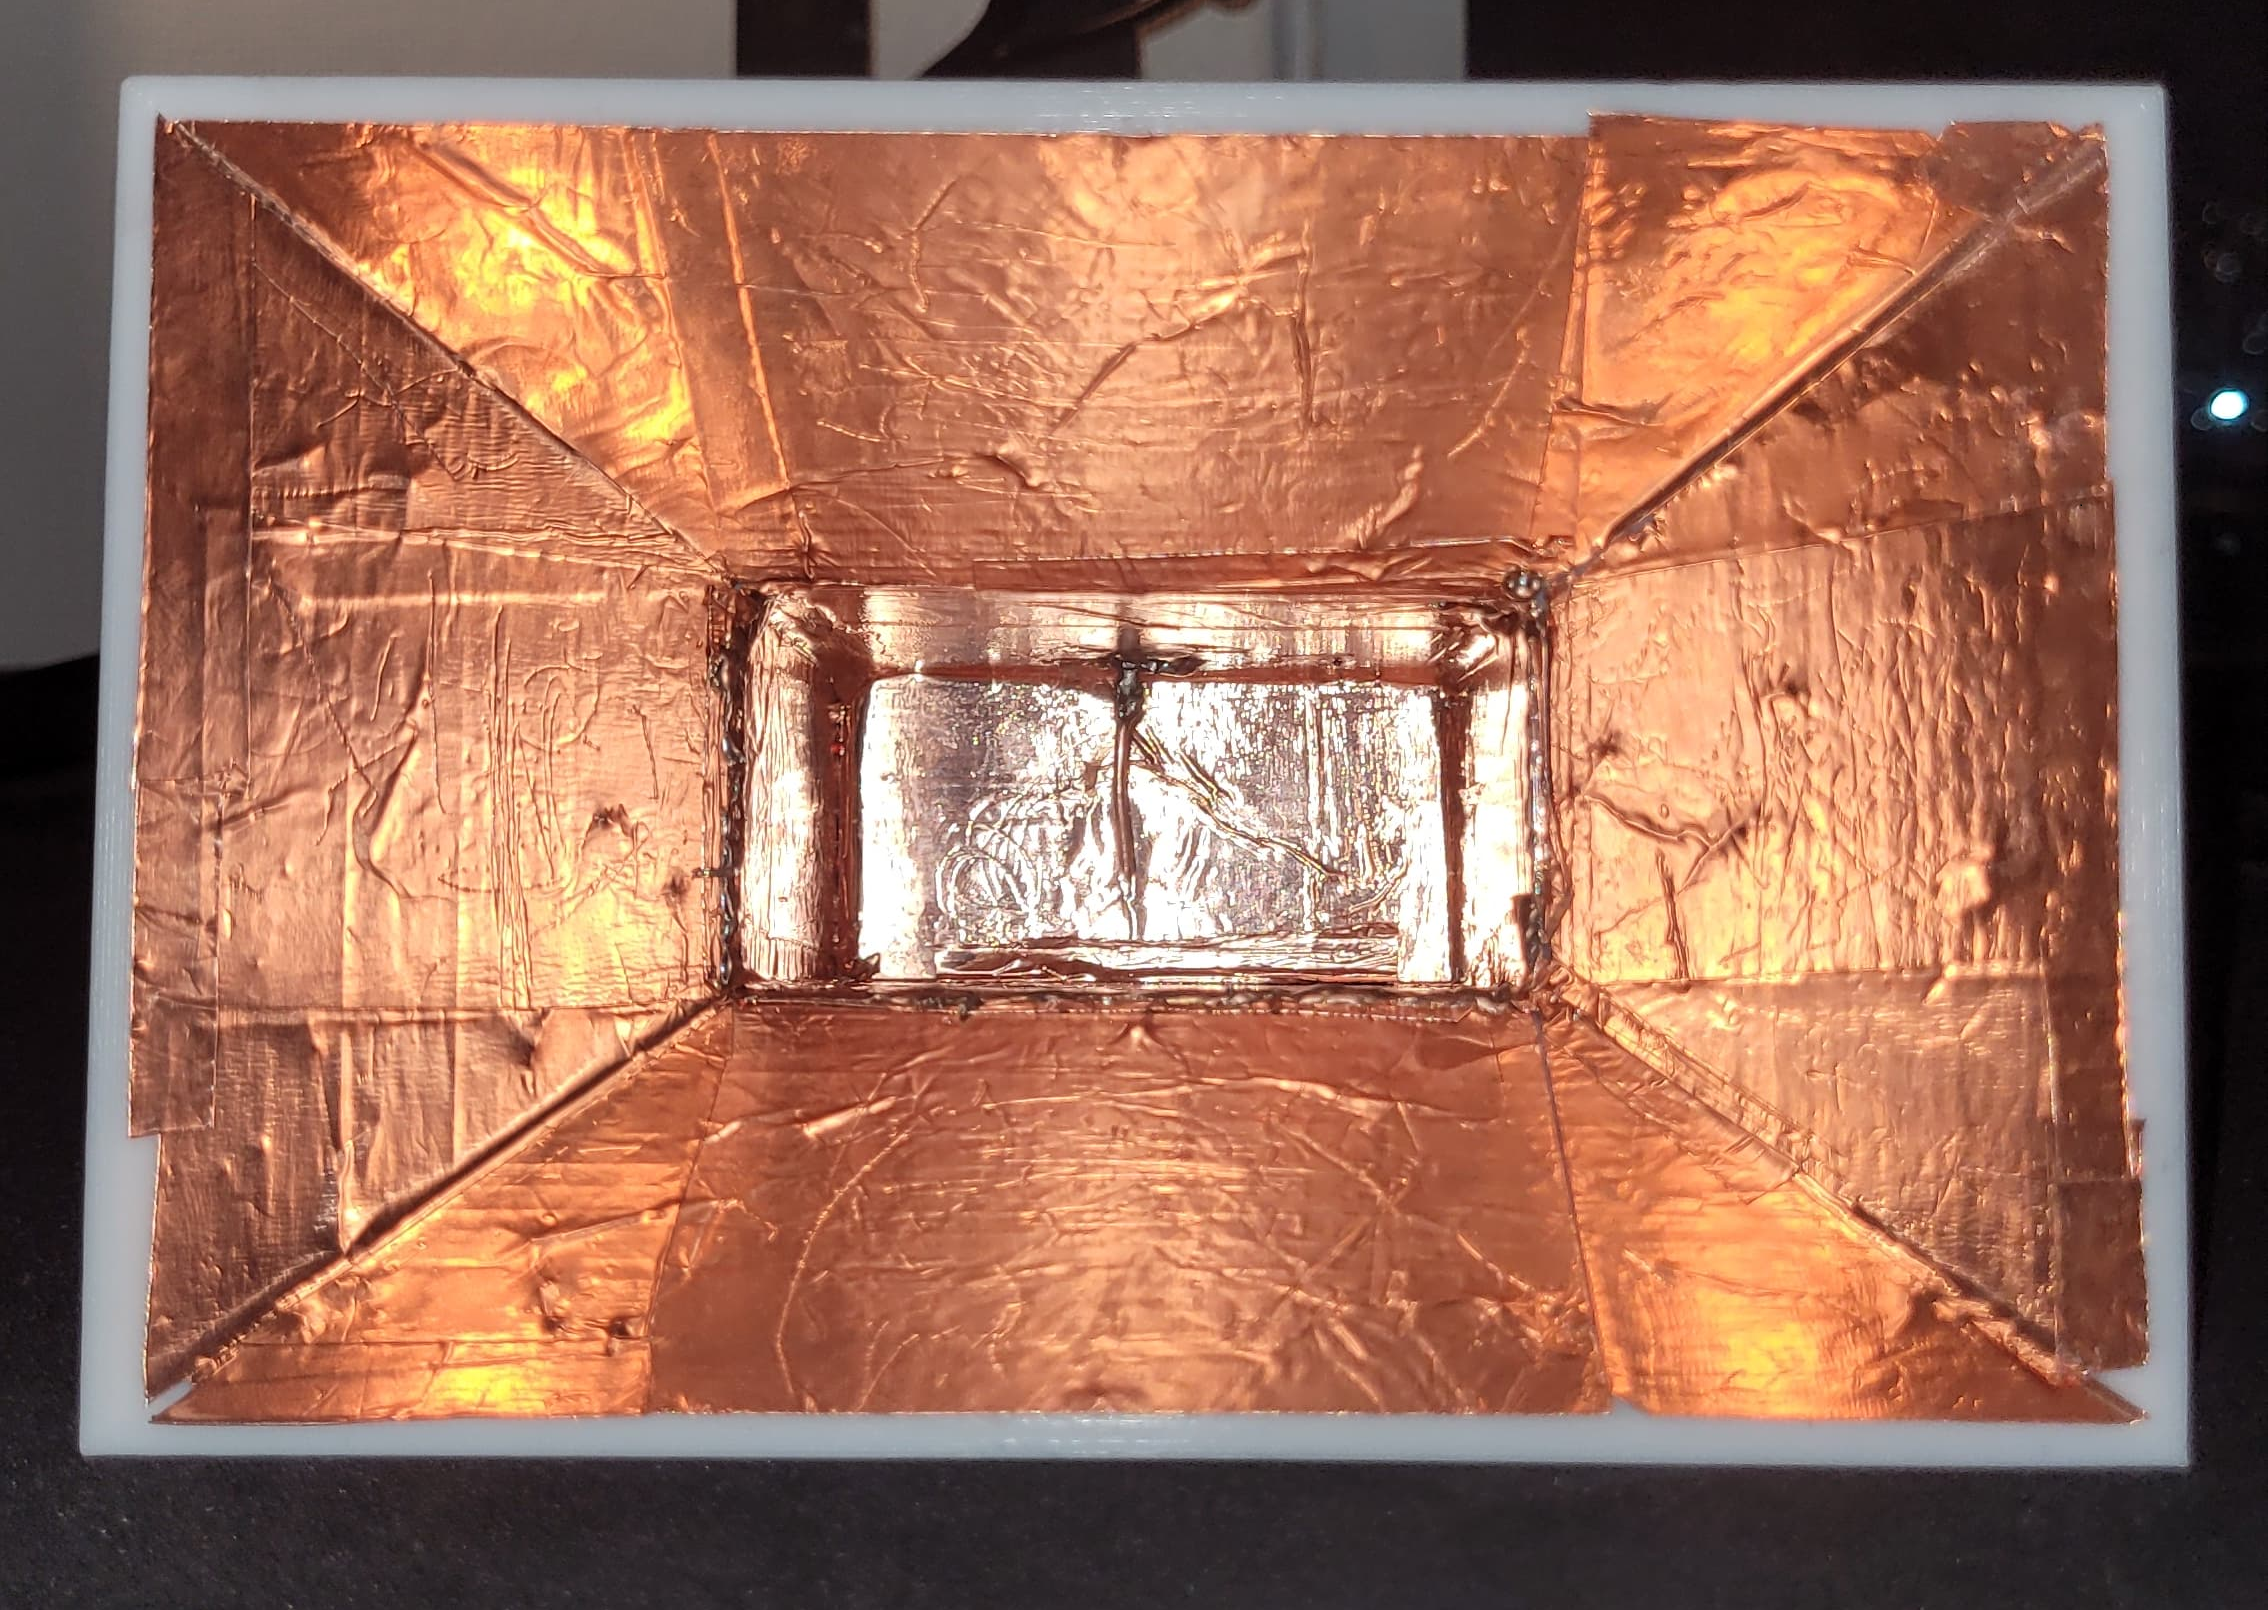
\includegraphics[width=0.8\textwidth]{img/Figure_7}
        \caption{Implementación del controlador difuso en \textit{Simulink} donde se considera el bloque \textit{Fuzzy Logic}, además de los ponderadores o ganancias \(GE\), \(GDE\) y \(GU\).}
        \label{fig:6}
    \end{figure}
    
    Luego se deben definir tanto las reglas asociadas al controlador difuso como los conjuntos difusos para cada premisa y para cada consecuencia en la construcción de las reglas. Se definen los siguientes conjuntos difusos para cada premisa asociada al error, la derivada del error y por último la salida del controlador difuso.
    
    \begin{figure}
        \centering
        \includegraphics[width=0.6\textwidth]{img/Figure_6}
        \caption{Definición de los conjuntos difusos tanto para el error (\textbf{e}), la derivada del error (\textbf{de}) y por último la salida del controlador difuso (\textbf{u}).}
        \label{fig:7}
    \end{figure}
    
    Los rangos se visualizan de mejor manera en la siguiente tabla:
    
    \begin{table}[h]
        \centering
        \caption{Parámetros de las Funciones de Membresía para las Variables de Entrada y Salida}
        \begin{tabular}{|c|c|c|c|}
        \hline
        \textbf{Variable} & \textbf{Conjunto Difuso} & \textbf{Tipo} & \textbf{Parámetros} \\ \hline
        \multirow{3}{*}{Error (\(e\))} & N (Negativo) & Triangular & \([-3, -2, 0]\) \\ \cline{2-4} 
         & Z (Cero) & Triangular & \([-1, 0, 1]\) \\ \cline{2-4} 
         & P (Positivo) & Triangular & \([0, 2, 3.667]\) \\ \hline
        \multirow{3}{*}{Derivada del Error (\(de\))} & N (Negativo) & Triangular & \([-1, -1, 0]\) \\ \cline{2-4} 
         & Z (Cero) & Triangular & \([-0.5, 0, 0.5]\) \\ \cline{2-4} 
         & P (Positivo) & Triangular & \([0, 1, 1]\) \\ \hline
        \multirow{3}{*}{Salida (\(u\))} & N (Negativo) & Triangular & \([-1, -1, 0]\) \\ \cline{2-4} 
         & Z (Cero) & Triangular & \([-0.5, 0, 0.5]\) \\ \cline{2-4} 
         & P (Positivo) & Triangular & \([0, 1, 1.833]\) \\ \hline
        \end{tabular}
    \end{table}
    
    Luego, se deben definir las reglas difusas asociadas al controlador difuso, las cuales se muestran en la siguiente tabla:
    
    \begin{table}[h]
        \centering
        \caption{Reglas de Inferencia para el Controlador Difuso PI}
        \begin{tabular}{|c|c|c|c|}
        \hline
        \textbf{Regla} & \textbf{Condición} & \textbf{Resultado} & \textbf{Salida (u)} \\ \hline
        1 & Si \(e\) es N y \(de\) es N & Entonces \(u\) es & N \\ \hline
        2 & Si \(e\) es N y \(de\) es Z & Entonces \(u\) es & N \\ \hline
        3 & Si \(e\) es N y \(de\) es P & Entonces \(u\) es & Z \\ \hline
        4 & Si \(e\) es Z y \(de\) es N & Entonces \(u\) es & P \\ \hline
        5 & Si \(e\) es Z y \(de\) es Z & Entonces \(u\) es & Z \\ \hline
        6 & Si \(e\) es Z y \(de\) es P & Entonces \(u\) es & N \\ \hline
        7 & Si \(e\) es P y \(de\) es N & Entonces \(u\) es & Z \\ \hline
        8 & Si \(e\) es P y \(de\) es Z & Entonces \(u\) es & P \\ \hline
        9 & Si \(e\) es P y \(de\) es P & Entonces \(u\) es & P \\ \hline
        \end{tabular}
    \end{table}
    
    Una vez implementado todo lo anterior asociado al controlador difuso, se obtiene la siguiente salida de la planta controlada.
    
    \begin{figure}
        \centering
        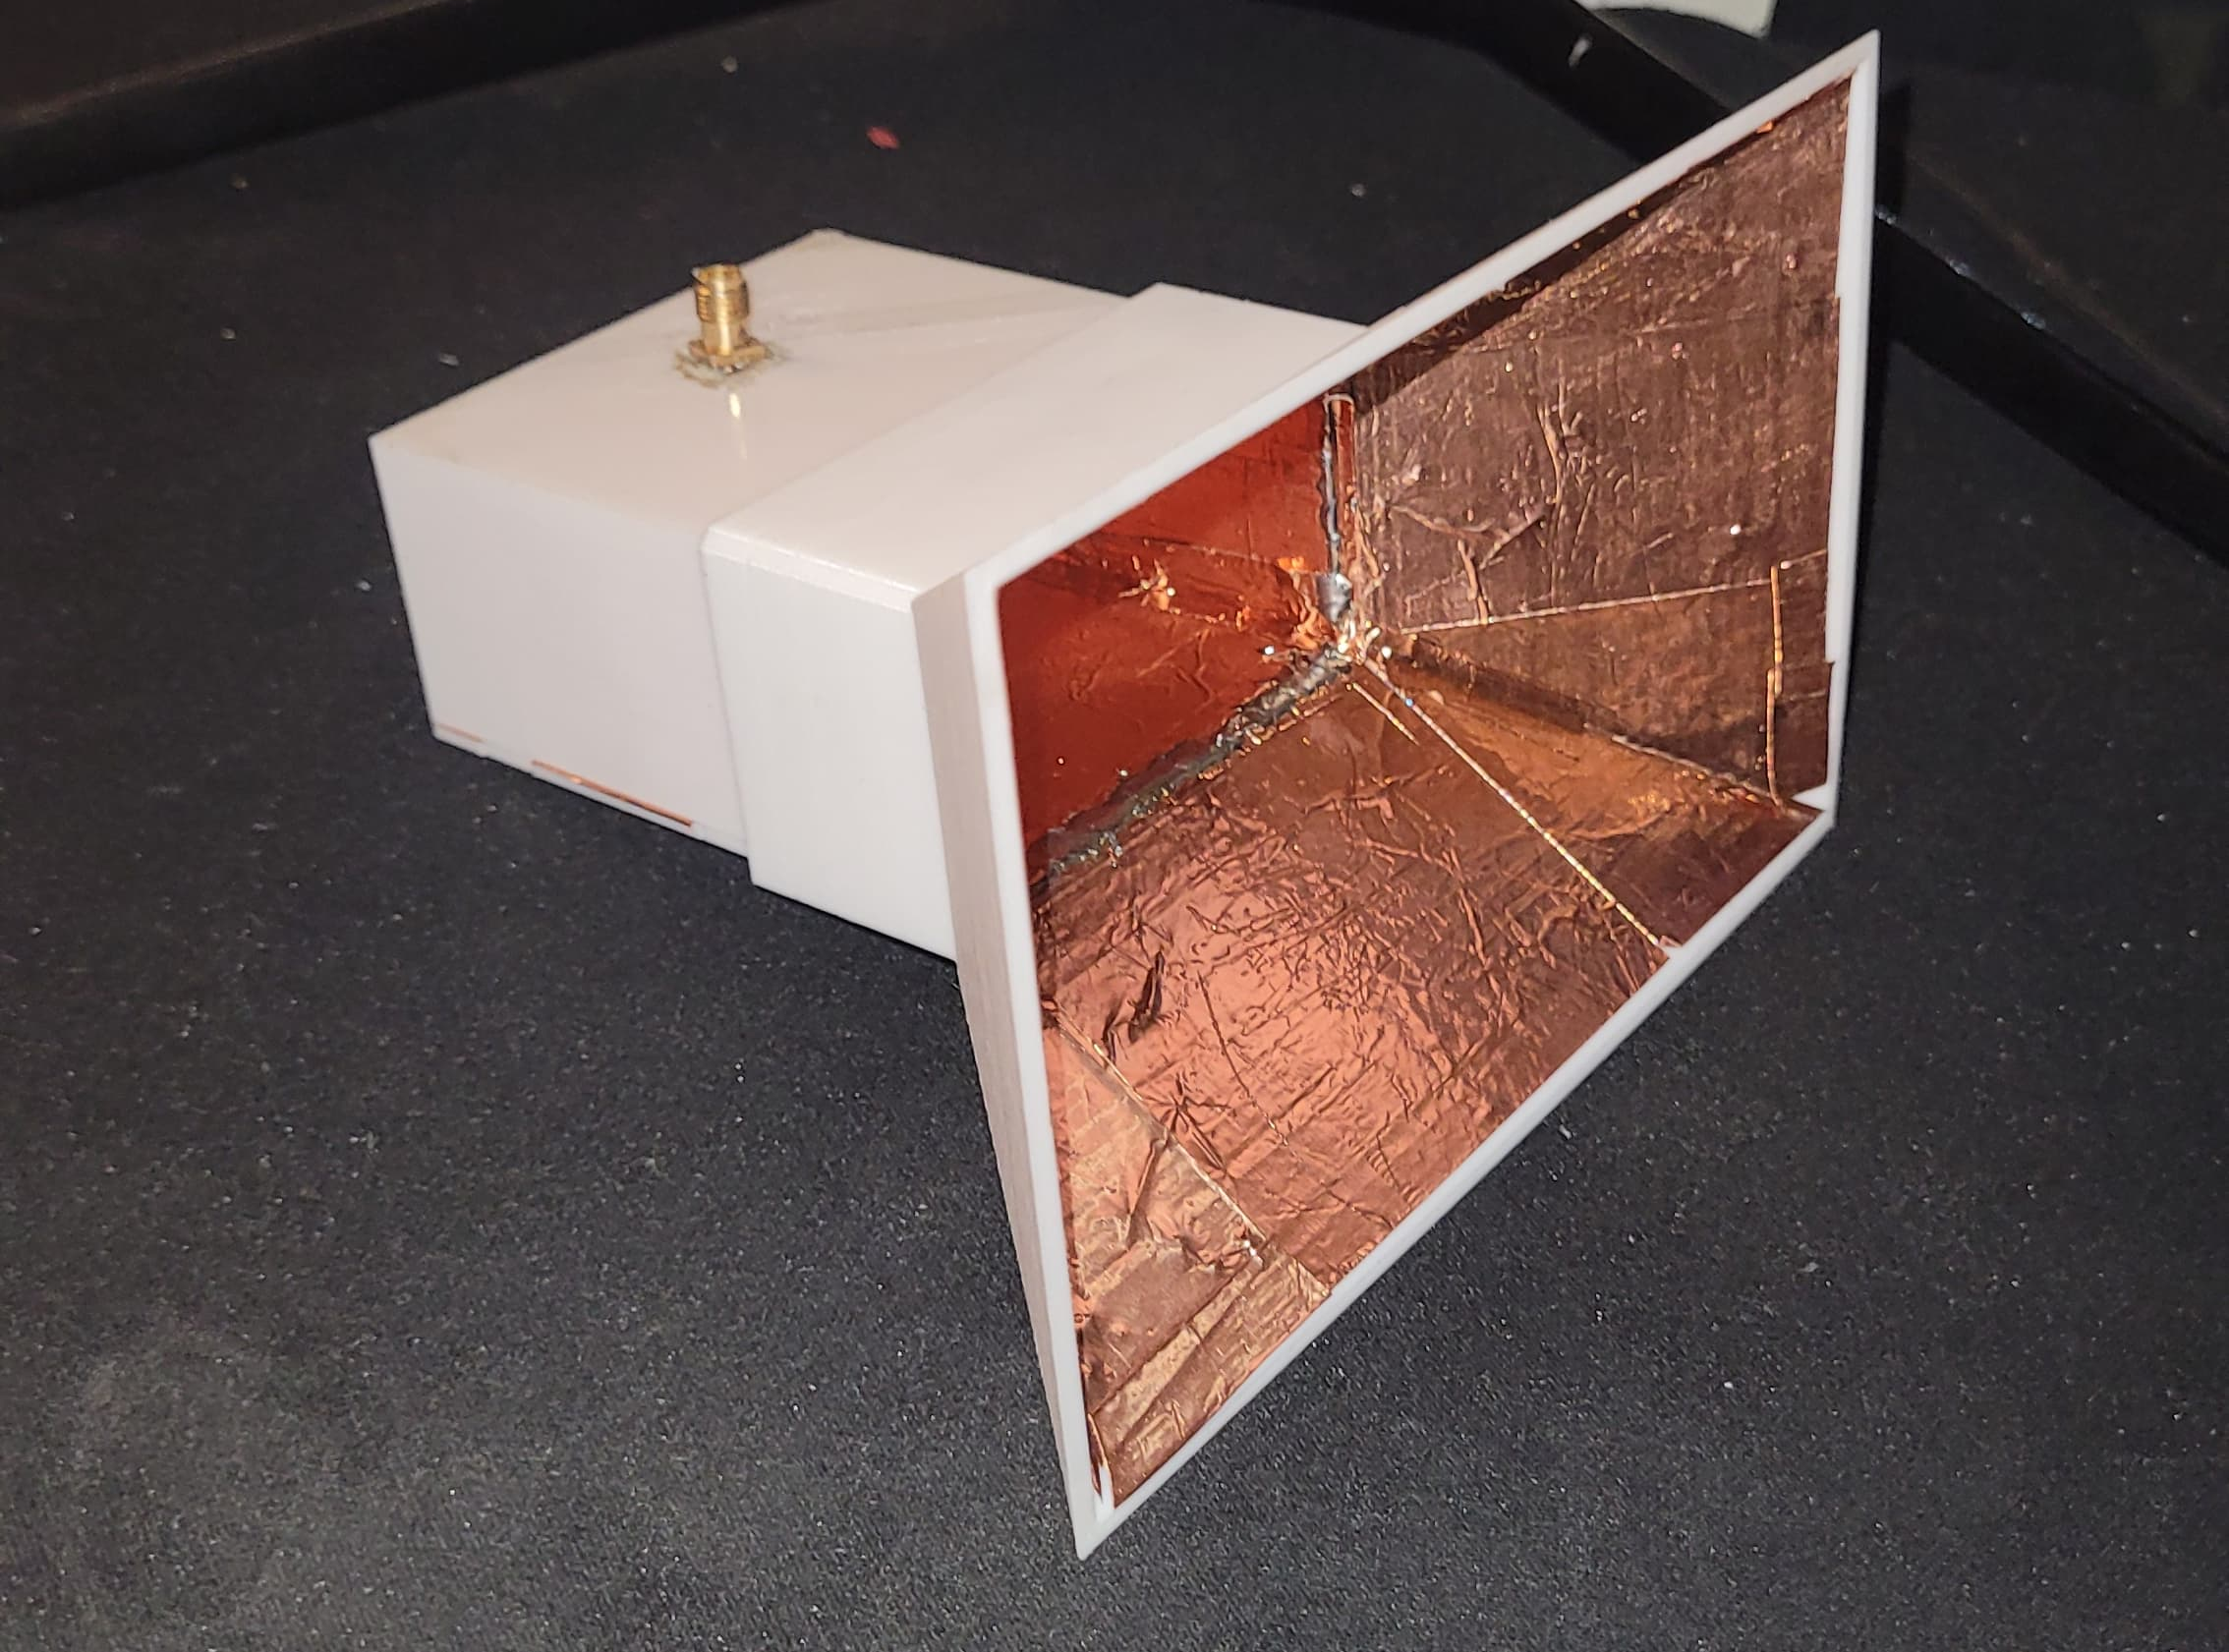
\includegraphics[width=0.7\textwidth]{img/Figure_8}
        \caption{Salida de la planta controlada donde se observa una respuesta suficientemente aceptable.}
        \label{fig:8}
    \end{figure}
    
    Finalmente, se puede concluir que el controlador PI difuso cumple con los requisitos de diseño y muestra una respuesta aceptable.
    \newpage
    \item \textbf{Diseñe e implemente un controlador MPC basado en un modelo ARX, indicando su estructura completa y probando con distintos parámetros de sintonización}. 
    
    Ahora se procederá a diseñar un controlador MPC basado en un modelo ARX. Para obtener los parámetros del modelo, se utiliza una señal PRBS en la entrada del sistema. La estructura básica se muestra en la Figura \ref{fig:9}.
    
    \begin{figure}
        \centering
        \includegraphics[width=0.75\textwidth]{img/Figure_10}
        \caption{Implementación de la señal PRBS en \textit{Simulink} para la obtención del modelo ARX.}
        \label{fig:9}
    \end{figure}
    
    Luego, se registran las respuestas de la planta a la señal PRBS, como se ilustra en la Figura \ref{fig:10}.
    
    \begin{figure}
        \centering
        \includegraphics[width=0.75\textwidth]{img/Figure_9}
        \caption{Señal PRBS y la respuesta de la planta para la obtención del modelo ARX.}
        \label{fig:10}
    \end{figure}
    
    Mediante un script en \textit{MATLAB}, se realiza la identificación del modelo ARX, obteniendo los siguientes coeficientes para el modelo:
    
    \begin{figure}
        \centering
        \includegraphics[width=0.8\textwidth]{img/Figure_11}
        \caption{Implementación del modelo ARX con sus parámetros óptimos y comparación de datos.}
        \label{fig:11}
    \end{figure}
    
    Los coeficientes obtenidos son los siguientes:
    
    \begin{table}[h]
        \centering
        \caption{Coeficientes del Modelo ARX}
        \begin{tabular}{|c|c|c|}
        \hline
        \textbf{Orden} & \textbf{Coeficientes A (Salida)} & \textbf{Coeficientes B (Entrada)} \\ \hline
        1 & -0.2229 & 0.9953 \\ \hline
        2 & 0.6442  & 0.2711 \\ \hline
        3 & 0.3981  & -0.0153 \\ \hline
        4 & 0.0495  & 0.0596 \\ \hline
        5 & 0.0470  & -0.0211 \\ \hline
        \end{tabular}
    \end{table}
    
    Finalmente, se implementa el controlador MPC en \textit{Simulink} utilizando los coeficientes del modelo ARX, como se muestra en la Figura \ref{fig:12}.
    
    \begin{figure}
        \centering
        \includegraphics[width=0.8\textwidth]{img/Figure_12}
        \caption{Implementación del controlador MPC en \textit{Simulink} con los coeficientes del modelo ARX.}
        \label{fig:12}
    \end{figure}
    
    Se concluye que el controlador MPC proporciona una respuesta aceptable, aunque presenta algunos sobresaltos que deben considerarse para mejorar la estabilidad y precisión del sistema.
    \item \textbf{Comparar el desempeño de los 3 controladores anteriores cuando ocurre un cambio en la referencia. Haga referencia a las métricas que considere pertinente. En particular, utilice la siguiente referencia:}

    \[
    r(t) = 
    \begin{cases} 
    2 & t \leq 200 \; [\text{s}] \\ 
    5 & 200 \leq t < 400 \; [\text{s}] \\ 
    8 & 400 \leq t \leq 600 \; [\text{s}]
    \end{cases}
    \]
    Dado que se busca comparar el desempeño de los controladores, se considerara diferentes escalones, por lo que implementara de la siguiente manera:
    \begin{figure}
        \centering
        \includegraphics[width=0.8\textwidth]{img/Figure_13}
        \caption{Implementación de la señal de referencia \(r(t)\) en \textit{Simulink} para la comparación de los controladores.}
        \label{fig:13}
    \end{figure}
    Luego tendremos que la respuesta para el controlador PI clásico es la siguiente:
    \begin{figure}
        \centering
        \includegraphics[width=0.8\textwidth]{img/Figure_14}
        \caption{Respuesta del controlador PI clásico para la señal de referencia \(r(t)\).}
        \label{fig:14}
    \end{figure}
    Para el controlador PI difuso, se obtiene la siguiente respuesta:
    \begin{figure}
        \centering
        \includegraphics[width=0.8\textwidth]{img/Figure_15}
        \caption{Respuesta del controlador PI difuso para la señal de referencia \(r(t)\).}
        \label{fig:15}
    \end{figure}
    Finalmente tenemos que para el controlador MPC, se obtiene la siguiente respuesta:
    \begin{figure}
        \centering
        \includegraphics[width=0.8\textwidth]{img/Figure_16}
        \caption{Respuesta del controlador MPC para la señal de referencia \(r(t)\).}
        \label{fig:16}
    \end{figure}
    Podemos comparar los graficos dando como resultado:
    \begin{figure}
        \centering
        \includegraphics[width=0.8\textwidth]{img/Figure_17}
        \caption{Comparación de las respuestas de los controladores para la señal de referencia \(r(t)\).}
        \label{fig:17}
    \end{figure}
    Se puede concluir que
\end{enumerate}
